\documentclass[11pt]{article}
\usepackage{amsmath}
%\usepackage{extsizes}
\usepackage{amsmath,amssymb}
%\usepackage{omegavn,ocmrvn}
%\usepackage[utf8x]{inputenc}
\usepackage[utf8]{vietnam}

\usepackage{listings}
\lstset{language=Python}          % Set your language (you can change the language for each code-block optionally)


\usepackage{longtable}
\usepackage{answers}
\usepackage{graphicx}
\usepackage{array}
\usepackage{pifont}
\usepackage{picinpar}
\usepackage{enumerate}
\usepackage[top=3.0cm, bottom=3.5cm, left=3.5cm, right=2.5cm] {geometry}
\usepackage{hyperref}


\newtheorem{bt}{Câu}
\newcommand{\RR}{\mathbb R}
\Newassociation{sol}{Solution}{ans}
\newtheorem{ex}{Câu}
\renewcommand{\solutionstyle}[1]{\textbf{ #1}.}


\begin{document}
% \noindent

\begin{tabular*}
	{\linewidth}{c>{\centering\hspace{0pt}} p{.7\textwidth}}
	Trường ĐHKHTN, ĐHQGHN & {\bf Học Kỳ 2 (2021-2022)}
	\tabularnewline
	K64 TTƯD - Thầy Hà Phi & {\bf Bài Tập Giải Tích Số \\ \today}
	% Exercises on pages 239, 240 Cheney/Kincaid are really nice
	\tabularnewline
	\rule{1in}{1pt}  \small  & \rule{2in}{1pt} %(Due date:)
	\tabularnewline
	%  \tabularnewline
	%  &(Đề thi có 1 trang)
\end{tabular*}




\begin{center}
	{\bf Bài Tập Giải Tích Số. No 6a \\ Giải số phương trình vi phân}
\end{center}

Trong Bài Giảng chúng ta được học 5 phương pháp: Euler hiện/ẩn; Trung điểm hiện; Hình thang; Heun.


\begin{bt} Viết các hàm trong Python để tính tích phân dựa trên 5 phương pháp nói trên theo mẫu 
	%
	\begin{lstlisting}[frame=single] 
		def ten_phuong_phap(f,x0,xf,h):
		return y , x
	\end{lstlisting}
	%	 
	trong đó $f = f(x,y)$ là hàm, $x \in [x0,xf]$ là khoảng thời gian, $h$ là độ rộng mỗi bước và được cho trước. Chú ý các nút được sử dụng là cách đều, tức là $x_0<x_1<\dots<x_f$, $x_i = x_{i-1} + h$. 
\end{bt}

	
\begin{bt}
Xét bài toán giá trị ban đầu
%
\begin{equation*}
	y'(x) = \dfrac{1}{y^2(x)} \quad ; \  y(0) = 1. 
\end{equation*}
%
a) Tìm nghiệm chính xác của bài toán trên. \\
b) Hãy thử giải số trên đoạn $[0,10]$, em quan sát thấy điều gì xảy ra. 
\end{bt}

\begin{bt}
a) Kiểm tra rằng hàm số $y(t) = t^2/4$ là nghiệm của bài toán giá trị ban đầu
\begin{equation*}
y'(t) = \sqrt{y} \quad ; \  y(0) = 0. 
\end{equation*}
b) Viết: Hãy thực hiện hai bước để tính nghiệm xấp xỉ với bước $h = 0.2$ bằng cả 5 phương pháp nói trên. \\
c) Viết script trong Python áp dụng cả 2 phương pháp Euler ẩn và hiện với bước đi $h = 0.01$ để xác định nghiệm số. Vẽ đồ thị sai số tuyệt đối của hai phương pháp Euler ẩn/hiện. 
Từ đó suy ra bậc hội tụ của phương pháp.
\end{bt}

\begin{bt}
Cùng câu hỏi như Bài tập 2 cho bài toán giá trị ban đầu
\begin{equation*}
y'(x) = - 4y + x^2  \ \mbox{ với } \ x \in [0,10] \quad ; \  y(0) = 1. 
\end{equation*}
%
Cho nghiệm chính xác là 
%
\[
y = \dfrac{31}{32} e^{-4x} + \dfrac{1}{4} x^2 - \dfrac{1}{8} x + \dfrac{1}{32}
\]
%
a) Xây dựng phương pháp Trung điểm ẩn bằng việc áp dụng phương pháp Euler ẩn để tính xấp xỉ giá trị hàm số $y_{k+0.5}$ tại trung điểm $x_{k+0.5}$. \\
b) Viết: Hãy thực hiện hai bước để tính nghiệm xấp xỉ với bước $h = 0.1$ bằng cả 4 phương pháp Trung Điểm ẩn/hiện; Hình Thang, Heun. \\
b) Viết script trong Python áp dụng cả 4 phương pháp nói trên để xác định nghiệm số trên đoạn $[0,10]$. Vẽ đồ thị sai số tuyệt đối của 4 phương pháp trên.
Từ đó suy ra bậc hội tụ của các phương pháp.
\end{bt}




\begin{bt} Cho 1 con lắc đơn (single pendulum) có khối lượng m = 1, thanh không khối lượng dài = 1, gia tốc trọng trường g = 1. 
Chuyển động của con lắc với góc $q$ và vận tốc góc $p$ được mô tả bởi 1 hệ phương trình vi phân có dạng 
\begin{align*}
	& \dot{p}(t) = - \sin q(t), \quad \mbox{ với mọi } t\geq 0, \\
	&  \dot{q}(t) = p(t).
\end{align*}
%
Hàm năng lượng của hệ (Hamiltonian) có dạng $H(p,q) = \dfrac{1}{2} p^2 - \cos q$.
%
\begin{figure}[!h]
	\centering
	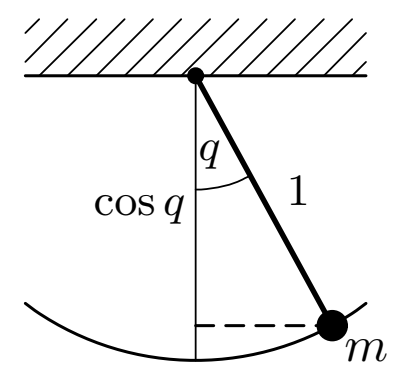
\includegraphics[width=0.3\linewidth]{Figures/pendulum}
	\caption{Single pendulum - Energy preserving method}
	\label{fig:pendulum}
\end{figure}
%

\noindent a) Chứng minh rằng $H(p,q)$ là hằng số dọc theo quỹ đạo nghiệm. \\
b) Hãy lập trình để kiểm tra xem trong 6 phương pháp nói đến ở các bài tập trên, phương pháp nào đảm bảo tính chất trong câu a)? Phương pháp đó được gọi là phương pháp bảo toàn năng lượng (energy preserving). Điều kiện ban đầu $p(0)$, $q(0)$ có thể chọn ngẫu nhiên.
\end{bt}

\centerline{———————————Hết——————————-}

\end{document}

\vspace{1cm}
\noindent{\bf Chú ý:} {\it Cán bộ coi thi không giải thích gì thêm}\\
\Closesolutionfile{ans}
\newpage
\begin{center}
{\LARGE{\bf ĐÁP ÁN}}
\end{center}

\begin{sol}
	\begin{figure}[h!]
		\centering
		\includegraphics[width=0.8\linewidth]{Solution1/Sol4_1.png}
		%\caption{}
		\label{fig:Sol4}
	\end{figure}
	Exercise 7: Convergence order is 3.	
\end{sol}

   
\end{document}



